\chapter{随机蕨算法的改造与应用}

\section{概述}

随机蕨算法是随机森林算法的一种变种,也是基于传统贝叶斯理论提出的一种集成学习方法,
最早由Mustafa Ozuysal等人提出\cite{ozuysal2007fast}。
随机蕨和随机森林的区别主要有如下这四个方面:
\begin{itemize}
\item
随机森林算法直接学习后验概率,
而随机蕨算法则是通过学习类别条件概率密度分布
\item
在随机森林算法中,对于每个输入样本,比较的特征次序会有所不同,
但是在随机蕨算法中,对于每个输入的样本比较的特征的次序都是相同的。
\item
在训练过程中,随机森林算法的训练时间是随着随机树的深度指数增长,
而在随机蕨算法中,训练时间仅仅随着数的深度呈线性增长。
\item
在随机森林算法中,算法的最后结果是通过对每个决策树的加权平均来得到的,但是在随机蕨算法中,最后结果则是以贝叶斯规则综合得到。
\end{itemize}
% \begin{itemize}
% \item
% 随机森林算法直接学习后验概率$P(C_k|F)$,
% 而随机蕨算法则是通过学习类别条件概率密度分布$P(F|C_k)$
% \item
% 在随机森林算法中,对于每个输入样本,比较的特征次序会有所不同,
% 但是在随机蕨算法中,对于每个输入的样本比较的特征的次序都是相同的。
% \item
% 在训练过程中,随机森林算法的训练时间是随着随机树的深度指数增长,
% 而在随机蕨算法中,训练时间仅仅随着数的深度呈线性增长。
% \item
% 在随机森林算法中,算法的最后结果是通过对每个决策树的加权平均来得到的,但是在随机蕨算法中,最后结果则是以贝叶斯规则综合得到。
% \end{itemize}
% 其中,$P$表述算法最后的概率输出结果,$C_k$表示算法分类器的目标类别,$F=\{f_1,f_2,...,f_N\}$表示输入算法的特征,下文同。
随机蕨算法经过实验验证,在相同层数的情况下,具有比随机森林更为优秀的分类能力以及抗过拟合能力,同时在计算效率上与随机森林不分上下,仅仅在模型存储上有较高的需求。因此随机蕨凭借出色的表现,得到了越来越多的关注。

但随机蕨算法目前的讨论都是在分类问题的基础上进行的,算法最后的结果也是在给定类别数目的情况下才能实现。但是在很多实际问题中,往往遇到的是回归问题,需要求解的目标空间往往是连续的,这个时候上述方法将不再适用。本文针对这样的情况,结合随机蕨的特性,借鉴随机森林算法改造应用到拟合回归问题中的方法,将随机蕨算法加以改造,使其也能适用于拟合回归问题。在此基础上,本文将进一步扩充随机蕨算法,通过增加一层掩码机制使其在输入特征有较大噪声的情况下也能有较强的鲁棒性,使算法能够在更多的应用场景中有更稳定的表现。

本章结构安排如下:2.2节介绍随机蕨算法通过修改输出函数表达式可以实现其在拟合回归问题中的应用。2.3节将介绍如何将掩码添加进随机蕨算法框架中,从而实现随机蕨算法在对抗大噪声情况下仍然具有较强的鲁棒性。最后在2.4节,本文通过将随机蕨算法应用到人脸对齐问题中,通过实验验证了改进后的随机蕨算法在回归问题中的可行性以及相比于普通拟合算法的鲁棒性,说明了该改进算法具有较强的实用性。



\section{随机蕨算法基本原理}
本节简要阐述一下随机蕨算法的具体原理。对于一个分类问题,需要计算各个类别间的概率分布:
\begin{equation}
	\arg\max_{k} P(C_k|f_1,f_2,...,f_N)
\end{equation}
其中,$P$表述算法最后的概率输出结果,$C_k$表示算法分类器的目标类别,$F=\{f_1,f_2,...,f_N\}$表示输入算法的特征。在贝叶斯规则下,上式等价于:
\begin{equation}
	\arg\max_{k} P(f_1,f_2,...,f_N|C_k)P(C_k)
\end{equation}
该式子表明一个后验概率与先验概率密度与相似函数的乘积成正比。然而对于一个高纬度的特征描述,或者说一个复杂的决策树输入样本,是很难计算出或者学习出相关联的相似度分布。或者说计算高维度的相似度分布是一件非常耗时耗资源的工作,在很多计算资源有限、计算实时要求高的应用场景中,计算高维特征相似度变得非常笨重,$P(f_1,f_2,...,f_N|C_k)$会非常难以求解。但如果假设在给定了目标类别的情况下,特征的各个维度之间是有一定的相互独立性的。这个时候,朴素贝叶斯理论可以对上述公式有如下简化:
\begin{equation}
	P(f_1,f_2,...,f_N|C_k)=\prod_{i=1}^N P(f_i|C_k)
\end{equation}
从而目标类别表达式为:
\begin{equation}
	Class(F)\equiv \arg\max_k P(C_k)\prod_{n=1}^N P(f_n|C_k)
\end{equation}
但这个独立性的假设在大多数的情况下是很难成立的,大多数情况下,上式得到的概率结果会小于真实的后验概率。为此,需要进一步假设。假设高维特征可以分解为几个小特征组合,并且这些小的特征组合之间是几乎完全相互独立的。这个假设在很多情况下都可以满足实用性。例如原始特征$F$分解为L组,每一组的特征大小为S,则有:
\begin{equation}
\begin{aligned}
	F=\{F_1,F_2,...,F_L\} \\
% \end{equation}
% \begin{equation}
	F_l=\{f_{l_1},f_{l_2},...,f_{l_S}\}
\end{aligned}
\end{equation}
当L组特征间相互独立假设下:
\begin{equation}
	P(f_1,f_2,...,f_N|C_k)=\prod_{l=1}^L P(F_l|C_k)
\end{equation}
于是可以得到最后的类别概率分布:
\begin{equation}
	Class(F_l)\equiv \arg\max_k P(C_k)\prod_{l=1}^L P(F_l|C_k)
\end{equation}
上式就是随机蕨算法的根本,采用半朴素贝叶斯的方式,平衡了算法计算的复杂性以及算法的准确性。其中每一个特征组构成的决策树被称为一个蕨,实际应用过程中,通过调整蕨的大小(也就是$S$的大小),就可以实现对算法复杂性以及准确性的控制。图2-1为该经典随机蕨算法的示意图。
\begin{figure}[htb]
	\centering 
	% 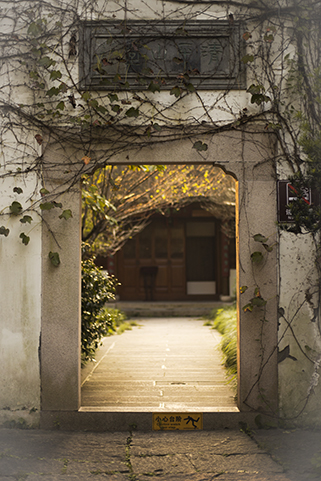
\includegraphics[width=\textwidth]{./Pictures/test.jpg} 
	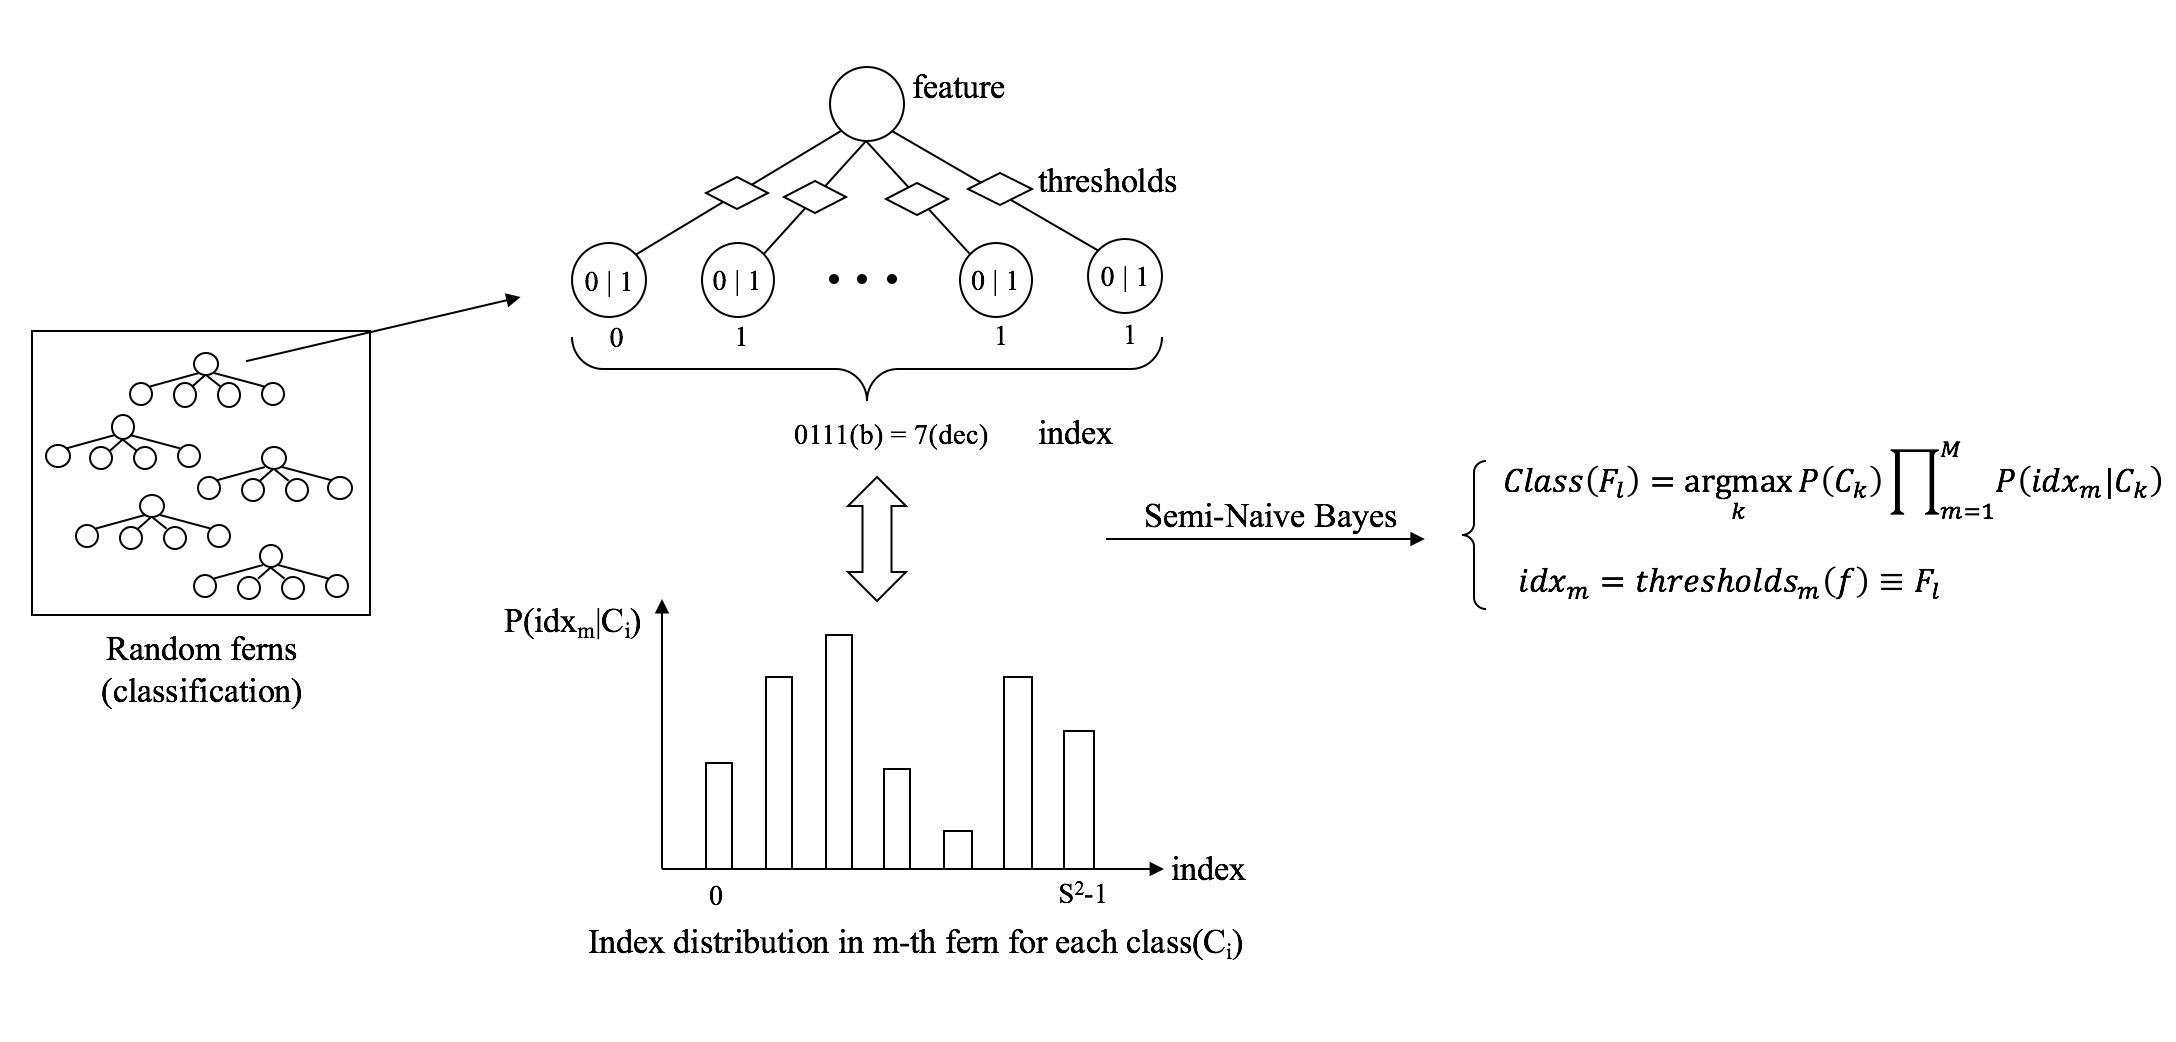
\includegraphics[width=\textwidth]{./mypic/经典随机蕨算法的示意图.jpg} 
	\caption{面向分类问题的经典随机蕨算法示意图} 
\end{figure}



\section{拟合回归问题下的随机蕨算法}
在分类问题下的随机蕨算法中,每个决策树的叶子节点记录的是所有落到该叶子节点的样本的类别概率分布均值。该模型在遇到新的输入样本后,将根据样本最后落入的叶子节点,统计所有叶子节点的概率分布均值来计算该样本的最后分类结果。这个模型显然不适用于回归问题。随机蕨算法被用于解决回归问题的思想最早在文章[\citenum{dollar2010cascaded}]中提出,后来也被应用到人脸对齐问题中\cite{cao2014face},但是都没有对其进行详细的说明阐述,很多算法实现细节被隐藏了。因此,本文将根据自己的理解和对算法的改善在此重新整理。

假定所有的输入样本都具有相同的特征维度$N$,$F=\{f_1,f_2,...,f_N\}$,以及相同$P$维度的目标回归空间$Y=\{y_1,y_2,...,y_P\}$。

首先任意地随机选取$S$个输入特征维度$(S<N)$,并随机生成$S$个阈值。将训练数据的这$S$个维度与这$S$个随机阈值进行简单大小比较,理想情况下可以得到$2^S$种不同的情况,同时对应地生成$2^S$个索引码。对这$2^S$个类别下的训练数据,我们计算其类内的均值,并记录为$L:\{L_1,L_2,...,L_{2^S}\}$,这样我们就得到了一个最简单的蕨。对于这个蕨,每次输入一个新的样本,仅仅需要将这个新的样本中那对应的$S$个维度上的数值与这$S$个阈值进行比较,就可以得到一个分类索引,然后只要根据这个索引在$L$中找到对应的均值记录(假定索引值为$i$),取出该均值便可以得到新样本的回归拟合值$L_i$。

这个基础蕨具有非常弱的拟合能力,甚至在随机阈值非常极端的情况下有可能完全不具备拟合能力。因此,我们需要重复这个随机过程(包括选取随机维度和生产随机阈值)多次,并记录下每一次随机过程的结果,并用损失函数来衡量这个随机过程得到的基础蕨的质量。损失函数可以有很多,例如:
\begin{equation}
	Loss=\sum_i{\|L_i-\overline{L_i}\|}
\end{equation}
如果某一次得到的损失函数值在所有随机过程中为最小,则抛弃所有其它的随机过程,用这次随机过程中选取的随机维度和随机阈值作为这个基础蕨的最终模型。记录维度信息$dim$、阈值信息$thresh$以及该阈值下的样本类别均值$L$。

这样的重复随机过程在经历一定量的次数之后将会大大加强该基础随机蕨的拟合能力,但是受限于随机过程的可重复次数,以及基础蕨的分类能力仅仅能实现$2^S$个,也限制了该基础蕨的拟合能力上限。因此,为了继续提高随机蕨算法的拟合能力,需要增加这种基础蕨的数量。区别于随机森林算法中各个树之间是相互独立的,随机蕨在生成众多的基础蕨过程中是有相互继承关系的。第一个基础蕨可以按上文所述进行生成,当生成第二个以及之后的基础蕨时,需要对每个样本的回归目标值进行修正,修正量就是上层基础随机蕨的预测结果。也就是说,第k层的回归目标值需要更新为:
\begin{equation}
	Y_{new}=Y_{original}-\sum_{i=0}^{k-1} Y_{pred_i}
\end{equation}
更新目标回归值之后,继续训练一定层数的随机蕨之后就可以得到最后具有非常高拟合能力的随机蕨模型。图2-2为该改进后的随机蕨回归算法的流程示意图。
\begin{figure}[htb]
	\centering 
	% 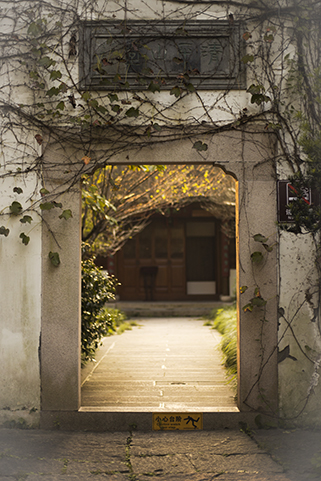
\includegraphics[width=\textwidth]{./Pictures/test.jpg} 
	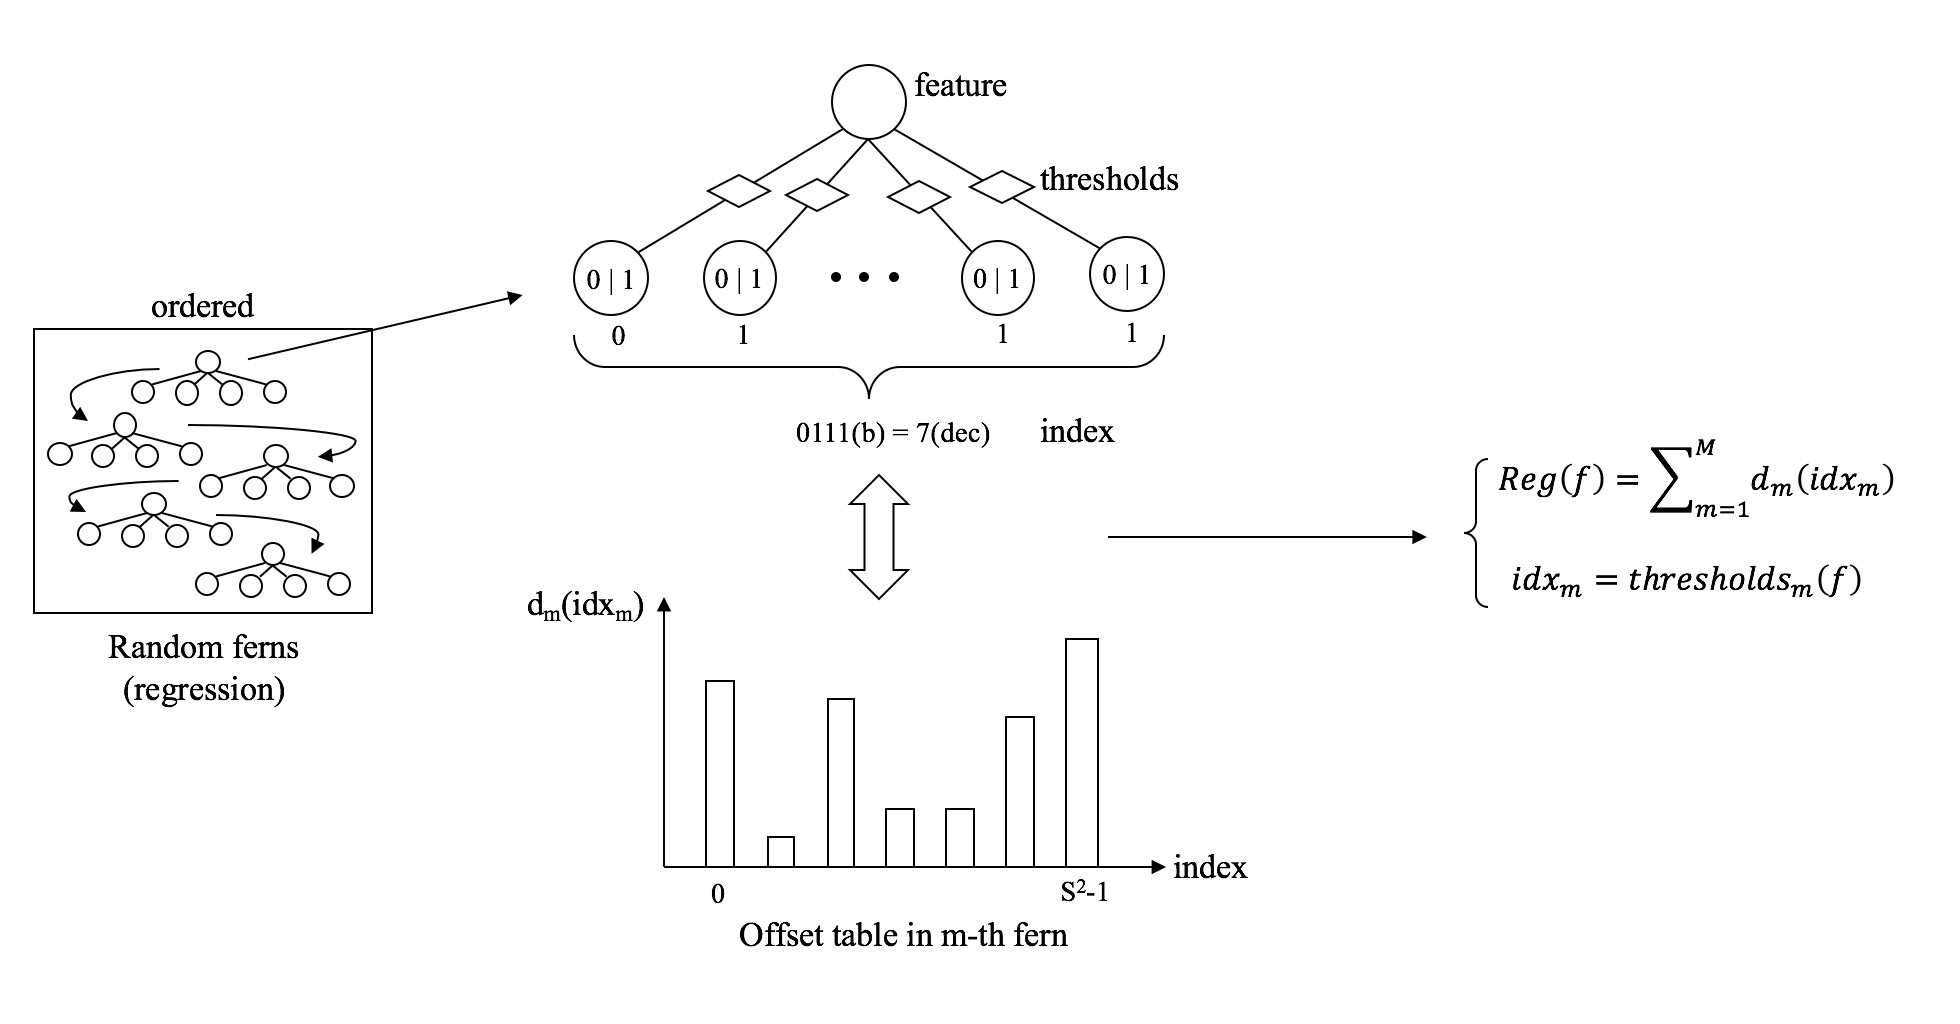
\includegraphics[width=\textwidth]{./mypic/改进后的随机蕨算法示意图.jpg} 
	\caption{改进后用于回归问题的随机蕨算法示意图} 
\end{figure}

上文表达了将随机蕨算法的核心思想,但是在实际实现该算法的时候仍将会遇到很多问题。过拟合问题是所有拟合算法中最常见的一种现象,这种现象也存在于随机蕨算法中。这一点可以通过在每一层基础蕨回归之后对每一层的回归量设置一个回归率,通过限制每一层的基础蕨的回归量上限可以非常好的抑制过拟合。虽然这种方法牺牲了一定的算法收敛速度,但是整体而言随机蕨回归算法仍旧有很高的计算速度。另外,在计算机代码实现过程中,随着随机蕨层数的增加,回归目标渐渐收敛,随机蕨的回归修正量会遇到浮点数的精度丢失问题。这个时候就需要利用额外记录每一层随机蕨回归目标均值作为保障。Algorithm 1 伪代码为随机蕨回归算法的整体概要。
% \newline
\newpage

\begin{algorithm}
\caption{随机蕨回归算法————训练模型 (Part I)}
\begin{algorithmic}[1]
\Require $D(data), L(label)$
\Require $S(depth), M(number\ of\ ferns), R(repeat\ times), eta(learning\ rate)$
\Ensure 随机蕨回归模型
\State 初始化:输入数据归一化等预处理;
\For{$M\ times$}
\Comment{随机蕨层数}
	\State $Loss_{min}\leftarrow MAX$
	\For{$R\ times$}
	\Comment{每层随机蕨重复随机过程次数}
		\State 随机产生S个维度与S个阈值:$dims, thresholds$
		\State $binary\ code=Compare(dims(D), thresholds)$
		\State \Comment 得到该基础蕨下所有训练样本的分类索引值
		\State 计算所有类内均值:$means$
		\State 更新所有训练样本的回归结果,计算$Loss$
		\If{$Loss<Loss_{min}$}
			\State 记录该基础蕨作为最佳基础蕨
% \algstore{bkbreak}
% \end{algorithmic}
% \end{algorithm}

% \begin{algorithm}
% \caption*{随机蕨回归算法————训练模型 (Part II)}
% \begin{algorithmic}[1]
% \algrestore{bkbreak}
			\State 保存该基础蕨的随机过程结果以及该随机过程下的训练样本分类均值
		\Else 
			\State $continue$
		\EndIf
	\EndFor
	\State $Y_{new}=Y_{original}-\sum_{i=0}^{m-1} Y_{pred_i}\cdot eta$
	\State \Comment 使用本次训练得到的最佳基础蕨的回归结果结合学习率更新回归目标
\EndFor
	% \State hh
\end{algorithmic}
\end{algorithm}


\begin{algorithm}
\caption{随机蕨回归算法————应用模型}
\begin{algorithmic}[1]
\Require $D(data)$,随机蕨回归模型
\Ensure $L(label)$
\State $Reg\leftarrow 0$
\Comment 初始化回归值
\For{$M\ times$}
\Comment{随机蕨层数}
	\State $binary\ code_m=Compare(dims_m(D), thresholds_m)$
	\Comment 得到本层基础随机蕨分类索引
	\State $reg_m=Indexing_m(binary\ code_m)$
	\Comment 得到本层基础随机蕨的回归值
	\State $Reg=Reg+reg_m$
	\Comment 将本次回归值累计到总回归值中去
\EndFor
\State \Return $Reg$
\end{algorithmic}
\end{algorithm}


% \newpage
% \pagebreak

\section{大噪声干扰下的随机蕨回归算法}

上一节中介绍了最基本的随机蕨回归模型,该模型在通常情况下都具有非常好的拟合能力,对于各种线性或者非线形问题都有很强的适应性。并且随机蕨回归算法在学习率的影响下,有非常好的抗过拟合能力,对轻微噪声也有很好的适应性。但是在实际应用过程中,会遇到一些数据极其不完备的情况。例如在一些回归问题中,输入的样本维度具有一定的不确定性,又或者在某些情况下输入样本的维度是一定的,但是有些维度的数据会存在严重噪声,如图2-3所示。

\begin{figure}[htb]
	\centering 
	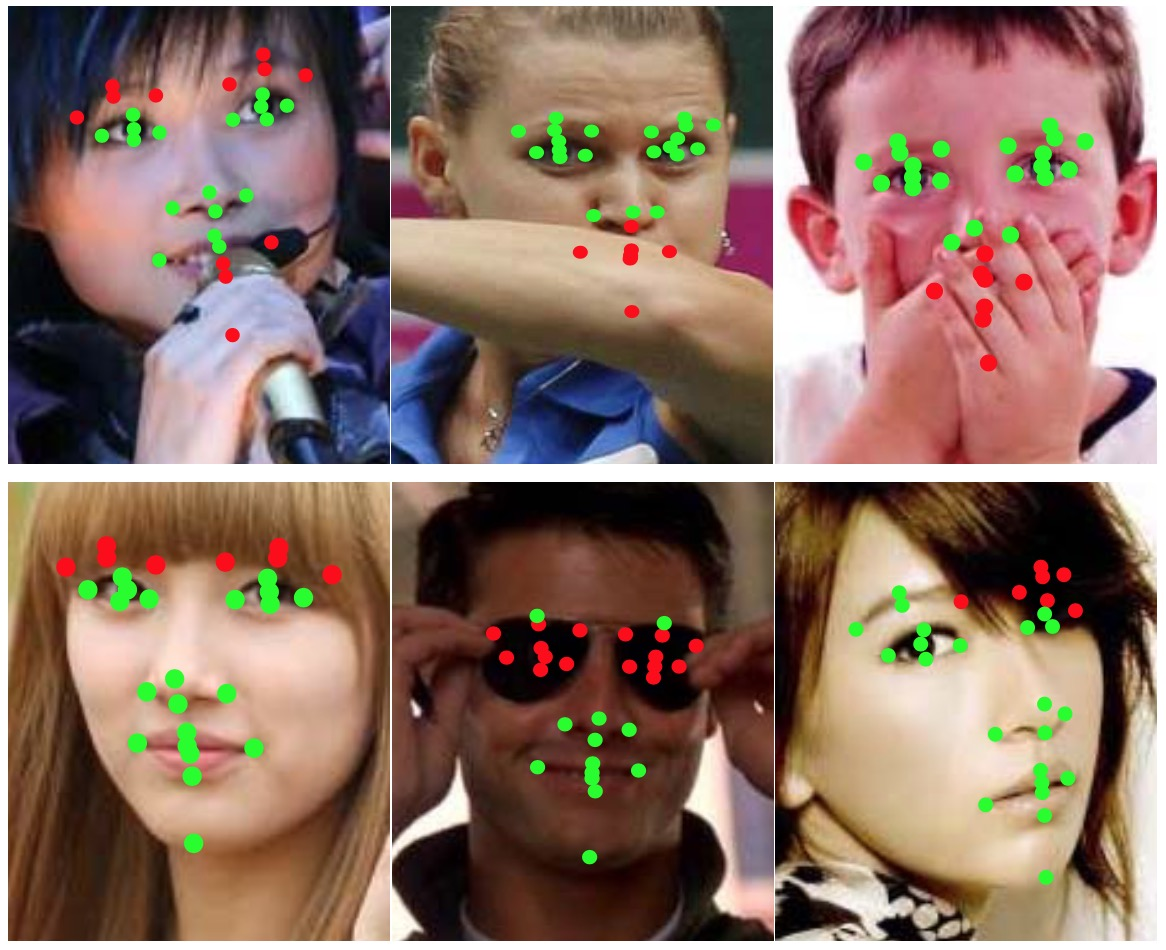
\includegraphics[width=0.7\textwidth]{./mypic/人脸特征由于被遮挡导致的缺失.jpg} 
	% 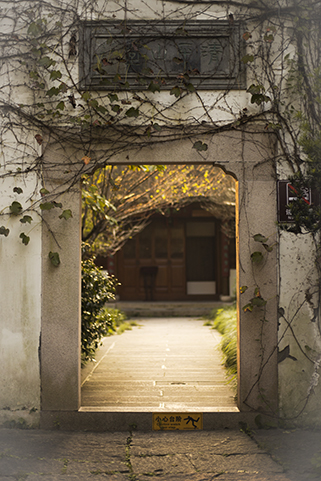
\includegraphics[scale=1.0]{./Pictures/test.jpg} 
	\caption{人脸特征(红点处)由于被障碍物遮挡导致缺失,缺失处的特征丧失了全部信息。} 
\end{figure}

这些情况下,在实验中会发现上节所述的随机蕨回归算法会遇到一个拟合能力严重不足的问题。例如存在一个输入样本特征描述$F=\{f_1,f_2,...,f_N\}$,其中有部分特征被噪声严重干扰,或者数据缺失,此时$F$为:
\begin{equation}
F=\{f_1,f_2,...f_p,f’_{p+1},...,f’_N\}
\end{equation}
其中$p+1$到$N$维特征为被噪声严重干扰的部分。这里注意随机蕨回归算法由于在选择特征维度的过程是完全随机的,不同样本也会有不同的被污染维度。例如在某一个样本中,前10个维度的特征被污染了,但是在另一个样本中后10个维度的特征被污染了,又或者在其他样本中完全随机的某些维度被污染。由于随机蕨算法中,每个基础蕨进行比较的那些维度($dims$)是完全随机生成的,因此为了方便后文阐述,上式中对于某一个样本,可以将被噪声严重污染的维度置于公式后方。

当特征存在上述被干扰情况的时候,从随机蕨算法中可以很容易看出,随机蕨算法存在两个缺陷。第一是当训练数据被干扰时,随机蕨回归模型在训练的过程中会尽量避免这些被污染的特征维度。因为一旦在随机过程中这些特征被选中,被污染的数据将会有错误的分类,并在最后分类均值的计算中严重干扰最后结果,最终导致整个随机蕨回归能力大大下降。第二是当随机蕨回归模型在训练的过程中并没有遇到严重的特征干扰问题,但是在实际应用过程中特征被大量污染以及干扰,这个时候被污染的特征维度直接导致样本的分类结果出现严重的偏差,就会导致最后的回归结果出现完全不在预期内的错误结果。

假设特征的被污染情况是可以被预测的(事实上在很多情况下这个假设是成立的,并且可以被很精确的估计),那么可以存在如下表达:
\begin{equation}
	B=\{b_1,b_2,...b_p,b_{p+1},...,b_N\}\in[0,1]
\end{equation}
其中$B$和$F$具有完全一致的维度,表示$F$的各个维度的置信度,也就是当$F$中某一维度的特征$F_i$被污染了的时候,对应的$B_i$将从百分之百可信度变为零(从1到0)。式(2-11)中假定第$1$到第$p$维都是未被污染的维度,第$p+1$到第$N$维都是被污染的维度,则有:
\begin{equation}
b_i=
\begin{cases}
1\quad {0\leq i\leq p} \\
0\quad {p<i\leq N}
\end{cases}
\end{equation}
$B$可以称为特征$F$的可信度掩码。在这个假设成立的情况下,我们可以充分利用这个信息来调整随机蕨回归算法。由于随机蕨算法中的每一个基础蕨都会根据出入特征的某几个维度进行回归,每个基础蕨在进行实际的回归之前可以先进行判断。如果该基础随机蕨要参考的那几个特征维度的可信度掩码值较低,则需要对这个随机蕨的回归量进行抑制,而当基础随机蕨参考的特征维度的可信度掩码值较高的时候,则对这个基础蕨的回归量不做调整。在算法实现过程中,特征维度的可信度掩码可以作为每个随机蕨的权值添加进算法中,也就是每个基础蕨的回归量应有如下表达:
\begin{equation}
	Reg_{fern}^{new} = Reg_{fern}^{original}\cdot f(B)
\end{equation}
其中$f(B)$为由可信度掩码生成的权值函数。在简单应用中,$f(B)$可以有简单的表达:
\begin{equation}
\begin{aligned}
	Q(i)=
	\begin{cases}
		1\quad i\in dims \\
		0\quad i\not\in dims
	\end{cases} \\
	f(B)=\frac{\sum_{i\in dims} b_i}{\sum_{i=0}^{N} Q(i)}
\end{aligned}
\end{equation}
在有了权值调整之后,当某一个基础蕨进行特征维度和阈值的比较时,会同时对可信度掩码进行处理。一旦输入的样本特征有较低的可行度时,$f(B)$将得到一个较低的值,从而抑制住这个基础蕨的回归量,避免杂乱的回归量对最后结果有较大的影响。并且这样处理仍然能让所有的维度都得到均匀的训练,不然被污染的维度会由于训练时$Loss$下降过少而被训练器忽略。同时在回归应用的时候,被污染的特征维度也会被抑制,保证最后回归结果不会因为某几个特征维度的干扰而破坏。

Algorithm 3 为增加掩码了机制的随机蕨算法的伪代码。
% \newline

\begin{algorithm}
\caption{掩码机制下的随机蕨回归算法————训练模型}
\begin{algorithmic}[1]
\Require $D(data), L(label), B(belief\ mask)$
\Require $S(depth), M(number\ of\ ferns), R(repeat\ times), eta(learning\ rate)$
\Ensure 随机蕨回归模型
\State 初始化:输入数据归一化等预处理;
\For{$M\ times$}
\Comment{随机蕨层数}
	\State $Loss_{min}\leftarrow MAX$
	\For{$R\ times$}
	\Comment{每层随机蕨重复随机过程次数}
		\State 随机产生S个维度与S个阈值:$dims, thresholds$
		\State $binary\ code=Compare(dims(D), thresholds)$
		\State \Comment 得到该基础蕨下所有训练样本的分类索引值
		\State $f(B)=\frac{\sum_{i\in dims} b_i}{\sum_{i=0}^{N} Q(i)}$
		\State \Comment 根据该基础蕨所选特征的置信度计算该基础蕨的回归量权值
		\State 计算所有类内均值:$means$
		\State $Y_{pred_i}=means(binary\ code)$
		\State $Y_{new}=Y_{original}-f(B)\cdot \sum_{i=0}^{m-1} Y_{pred_i}\cdot eta$
		\State \Comment 使用本次训练得到的基础蕨的回归结果结合学习率以及权值更新回归目标
		\State $Loss=\sum_i{\|Y_{new,i}-\overline{L_i}\|}$
		\State \Comment 计算$Loss$
		\If{$Loss<Loss_{min}$}
			\State 记录该基础蕨作为最佳基础蕨
			\State 保存该基础蕨的随机过程结果以及该随机过程下的训练样本分类均值
		\Else 
			\State $continue$
		\EndIf
	\State $\hat{Y}_{new}=\hat{Y}_{original}-\hat{f}(B)\cdot \sum_{i=0}^{m-1} \hat{Y}_{pred_i}\cdot eta$
	\State \Comment 使用最佳基础蕨的回归结果结合学习率以及权值更新回归目标
	\EndFor
\EndFor
\end{algorithmic}
\end{algorithm}

\begin{algorithm}
\caption{掩码机制下的随机蕨回归算法————应用模型}
\begin{algorithmic}[1]
\Require $D(data), B(belief\ mask)$,随机蕨回归模型
\Ensure $L(label)$
\State $Reg\leftarrow 0$
\Comment 初始化回归值
\For{$M\ times$}
\Comment{随机蕨层数}
	\State $binary\ code_m=Compare(dims_m(D), thresholds_m)$
	\Comment 得到本层基础随机蕨分类索引
	\State $reg_m=Indexing_m(binary\ code_m)$
	\Comment 得到本层基础随机蕨的回归值
	\State $Reg=Reg+reg_m$
	\Comment 将本次回归值累计到总回归值中去
\EndFor
\State \Return $Reg$
\end{algorithmic}
\end{algorithm}


\newpage

\section{实验结果与分析} % 人脸回归可以在这里写

为了验证随机蕨算法从分类问题下改进到回归问题下的合理性,本文进行了两个步骤的验证实验。首先通过一个基础拟合问题验证其基本的拟合能力,特别是对于非线性问题的拟合能力。然后在将其应用到人脸特征点定位这个高纬度、非线性的实际问题中,进一步验证其回归能力的鲁棒性。

\subsection{对随机蕨拟合能力的验证} %

首先验证随机蕨回归算法对于非线形问题的拟合能力,本文通过构造几个非线性函数,并添加随机噪声作为测试数据进行检验。

非线性函数具有如下表达式:
\begin{equation}
	f(x) = \cos(\lambda_1\pi x)+ \lambda_2 (x+1)^2 + \lambda_3 log(x+1) + \lambda_4
\end{equation}
其中包含三角函数项、多项式函数项、以及指数性质项,每给定任意的一组$\lambda_i$参数就可以得到一个特定的非线性函数。为了定量衡量算法回归能力,本文基于上述非线性函数,在自变量区间为$[0,1]$之间随机采样500个点,同时为函数值附加方差为$\sigma^2$的高斯噪声作为拟合模型的训练数据。最后将得到的拟合模型与原始函数进行比对,在同样自变量区间取1000个采样点,计算其与真值的方差$\hat{\sigma}^2$,以方差减少量作为拟合效果的评价指标。

表格2-1给出了其中20次随机实验的结果。实验中用于随机蕨拟合回归的训练参数为:学习率$eta=0.02$,$S=4$,$M=150$,$R=20$。从实验结果可以看出,原本存在较大方差噪声的数据经过随机蕨拟合回归之后,与原始模型相比方差减少幅度均值在95\%左右,对于非线性问题具有非常好的拟合能力。

图2-4给出了一些可视化数据。图中蓝色点表示用于训练随机蕨回归模型的训练数据点,红色点为随机蕨回归模型训练好之后预测的原始函数,绿色点表示原始函数真值。可以看到,图中红色点与绿色点已经非常接近,表明了随机蕨算法的拟合能力得到了验证。

\begin{table}[htb]
	\zihao{5}
	\caption{随机蕨拟合能力检验结果表} 
	% \label{Tabkeyword}
	\centering 
	\begin{tabular}[t]{
		% |c|l|r|p{4cm}|} 
		ccccccc} 
		\toprule
		$\lambda_1$ & $\lambda_2$ & $\lambda_3$ & $\lambda_4$ & 噪声方差 & 拟合后方差 & 方差减少幅度\\ 
		\midrule
		3.37292 & 0.649499 & 0.649499 & 0.649499 & 0.5 &    0.0124&    97.5229\% \\
		3.53833 & 0.792932 & 0.792932 & 0.792932 & 0.5 &    0.0153&    96.9383\% \\
		2.99967 & -0.525472 & -0.525472 & -0.525472 & 0.5 &    0.0119&    97.6265\% \\
		2.575 & 1.9678 & 1.9678 & 1.9678 & 0.5 &    0.0070&    98.6014\% \\
		2.15032 & 0.461065 & 0.461065 & 0.461065 & 0.5 &    0.0148&    97.0353\% \\
		3.09489 & -0.157773 & -0.157773 & -0.157773 & 0.5 &    0.0080&    98.3986\% \\
		5.09176 & 1.26823 & 1.26823 & 1.26823 & 0.5 &    0.0293 &    94.1431\% \\
		3.61479 & 1.71666 & 1.71666 & 1.71666 & 0.5 &    0.0133&    97.3352\% \\
		2.66396 & 1.1875 & 1.1875 & 1.1875 & 0.5 &    0.0102&    97.9562\% \\
		3.29159 & 1.72562 & 1.72562 & 1.72562 & 0.5 &    0.0160&    96.7915\% \\
		4.97152 & 0.308569 & 0.308569 & 0.308569 & 0.5 &    0.0430&    91.3997\% \\
		3.38681 & -1.90669 & -1.90669 & -1.90669 & 0.5 &    0.0102&    97.9517\% \\
		3.80523 & -1.54795 & -1.54795 & -1.54795 & 0.5 &    0.0108&    97.8402\% \\
		5.27595 & 0.855638 & 0.855638 & 0.855638 & 0.5 &    0.0287 &    94.2662\% \\
		2.22052 & 0.2368 & 0.2368 & 0.2368 & 0.5 &    0.0064&    98.7156\% \\
		5.79584 & -1.26993 & -1.26993 & -1.26993 & 0.5 &    0.0483&    90.3486\% \\
		2.42347 & -0.731821 & -0.731821 & -0.731821 & 0.5 &    0.0113&    97.7331\% \\
		4.42034 & 0.694184 & 0.694184 & 0.694184 & 0.5 &    0.0131&    97.3814\% \\
		4.83876 & 1.05292 & 1.05292 & 1.05292 & 0.5 &    0.0305&    93.8946\% \\
		\bottomrule
	\end{tabular}
\end{table}


\begin{figure}[htb]
	\centering 
	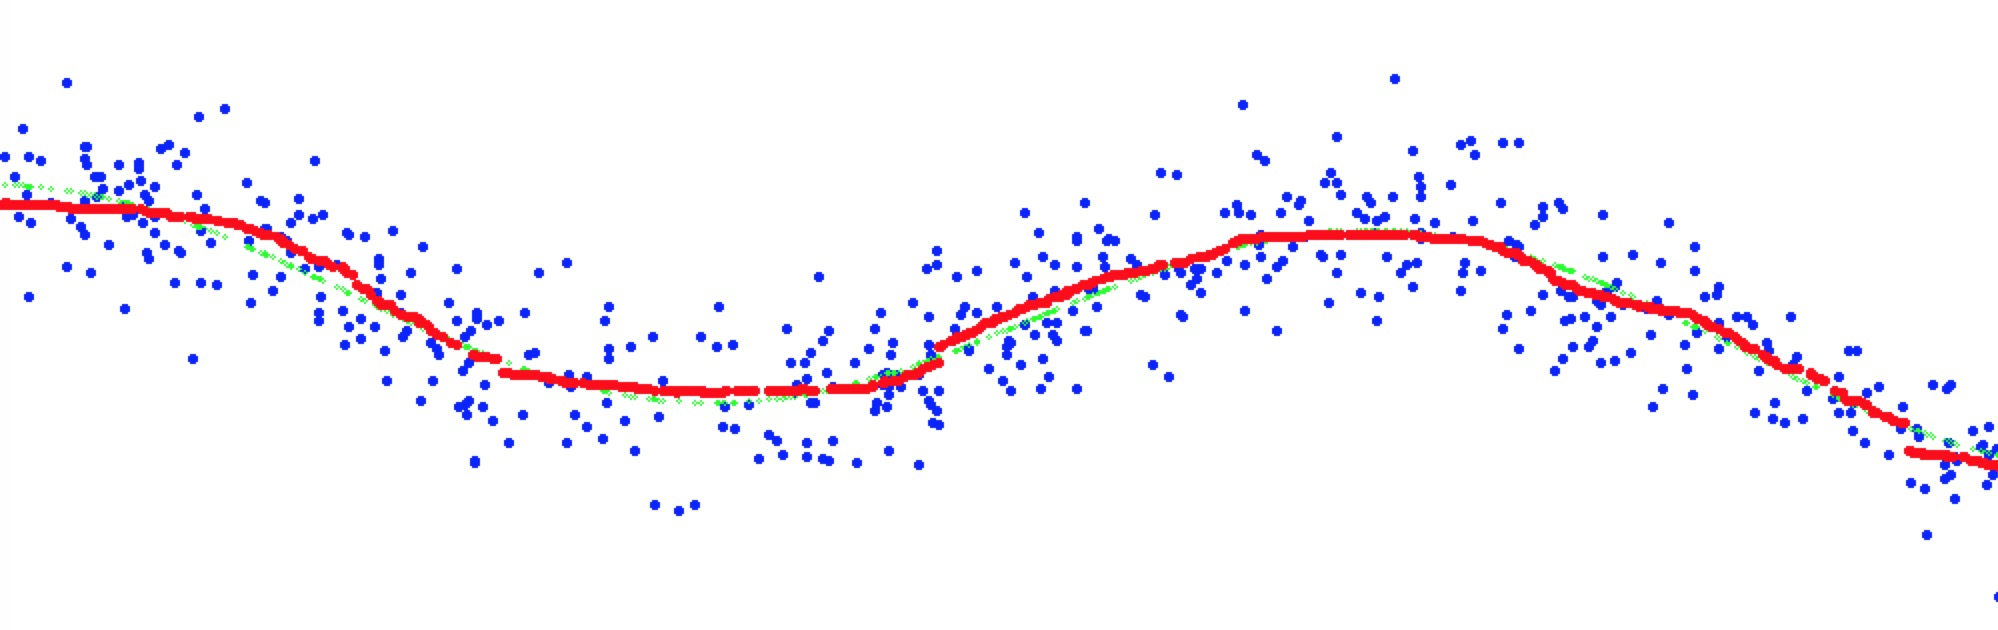
\includegraphics[width=0.6\textwidth]{./mypic/随机蕨回归实验1.jpg} 
	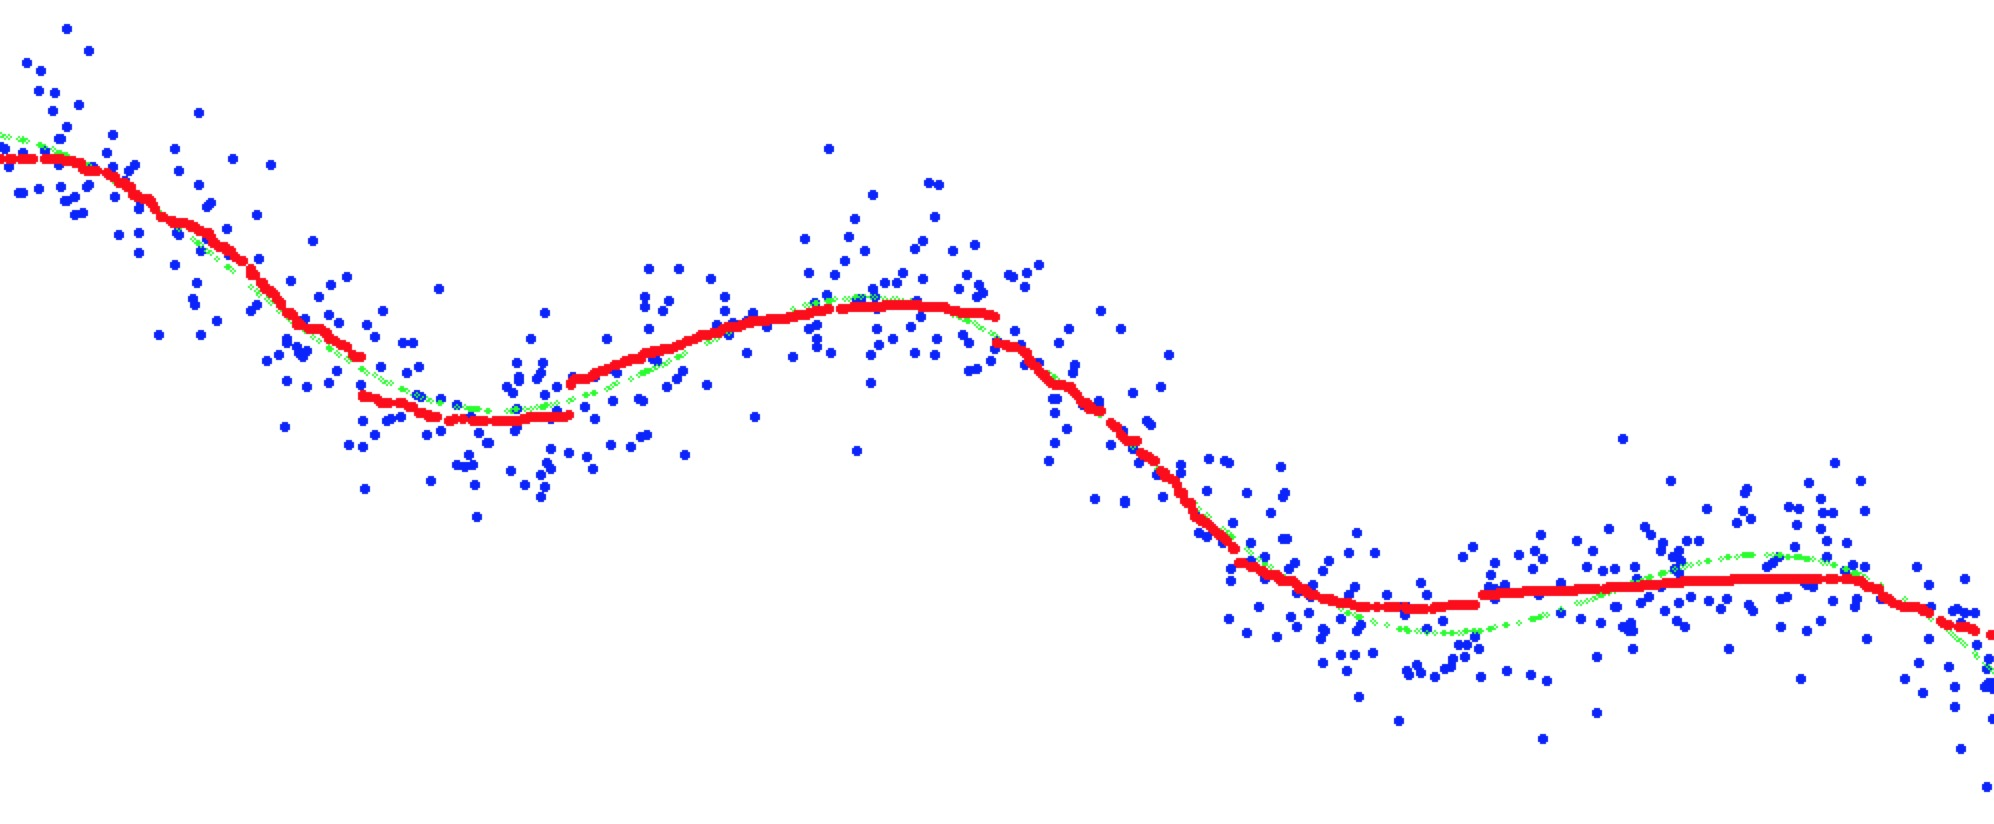
\includegraphics[width=0.6\textwidth]{./mypic/随机蕨回归实验2.jpg} 
	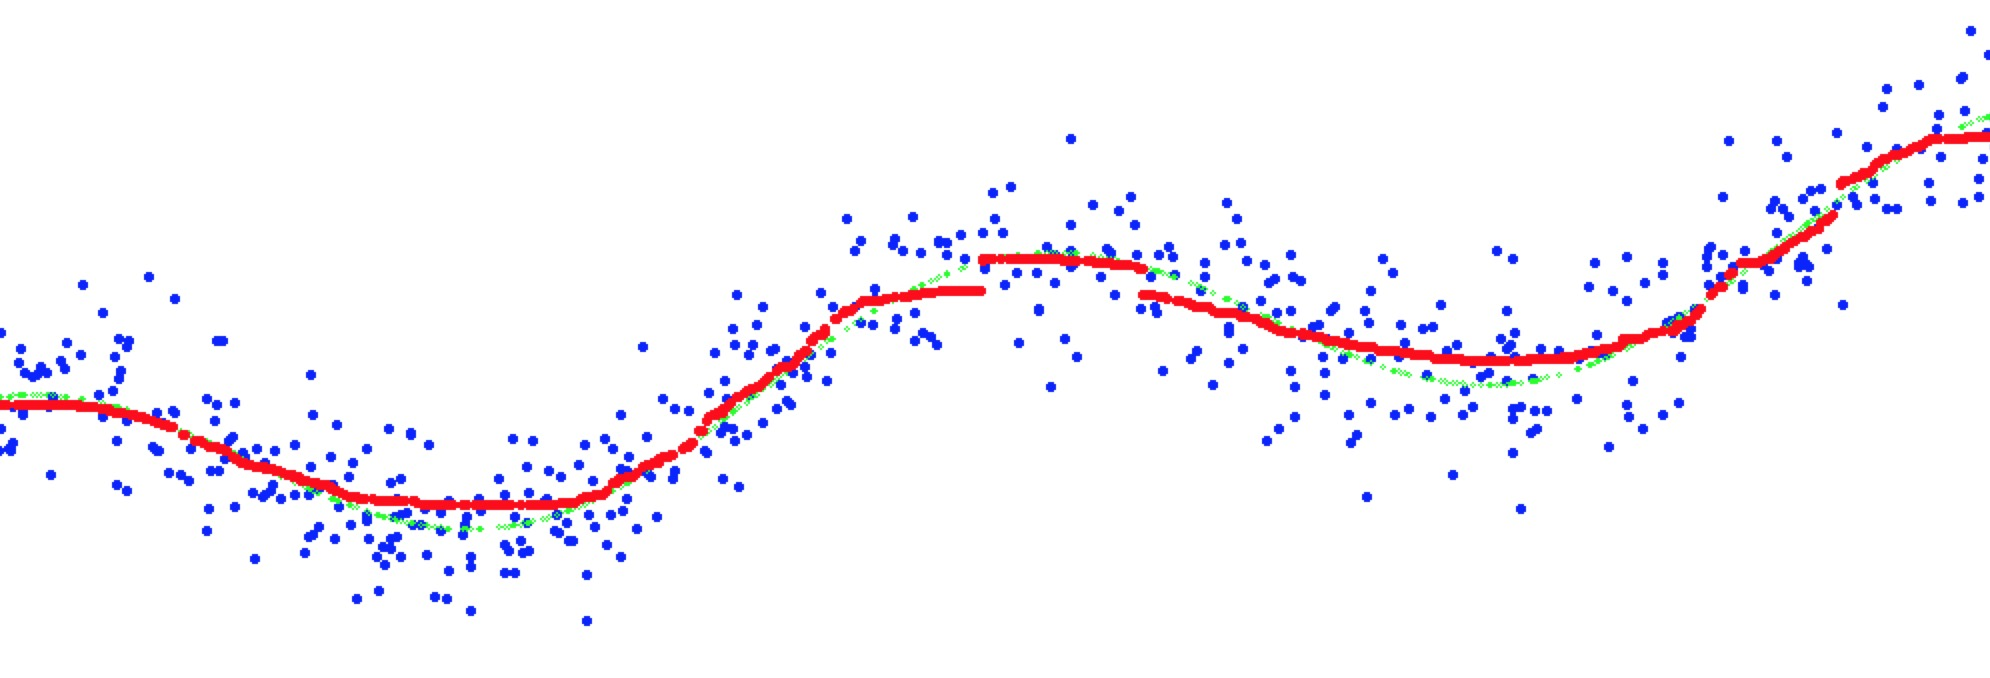
\includegraphics[width=0.6\textwidth]{./mypic/随机蕨回归实验3.jpg} 
	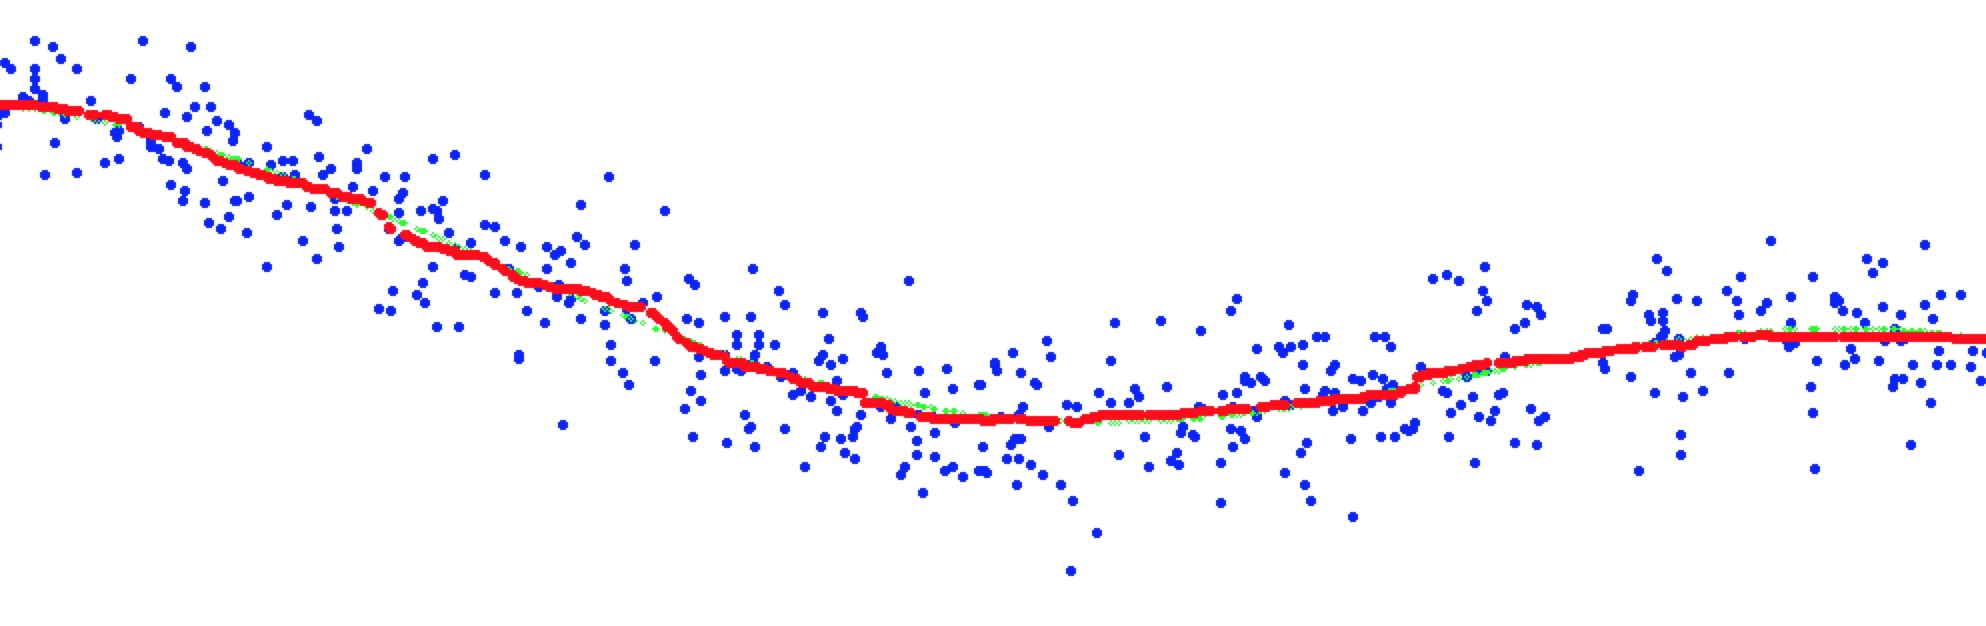
\includegraphics[width=0.6\textwidth]{./mypic/随机蕨回归实验4.jpg} 
	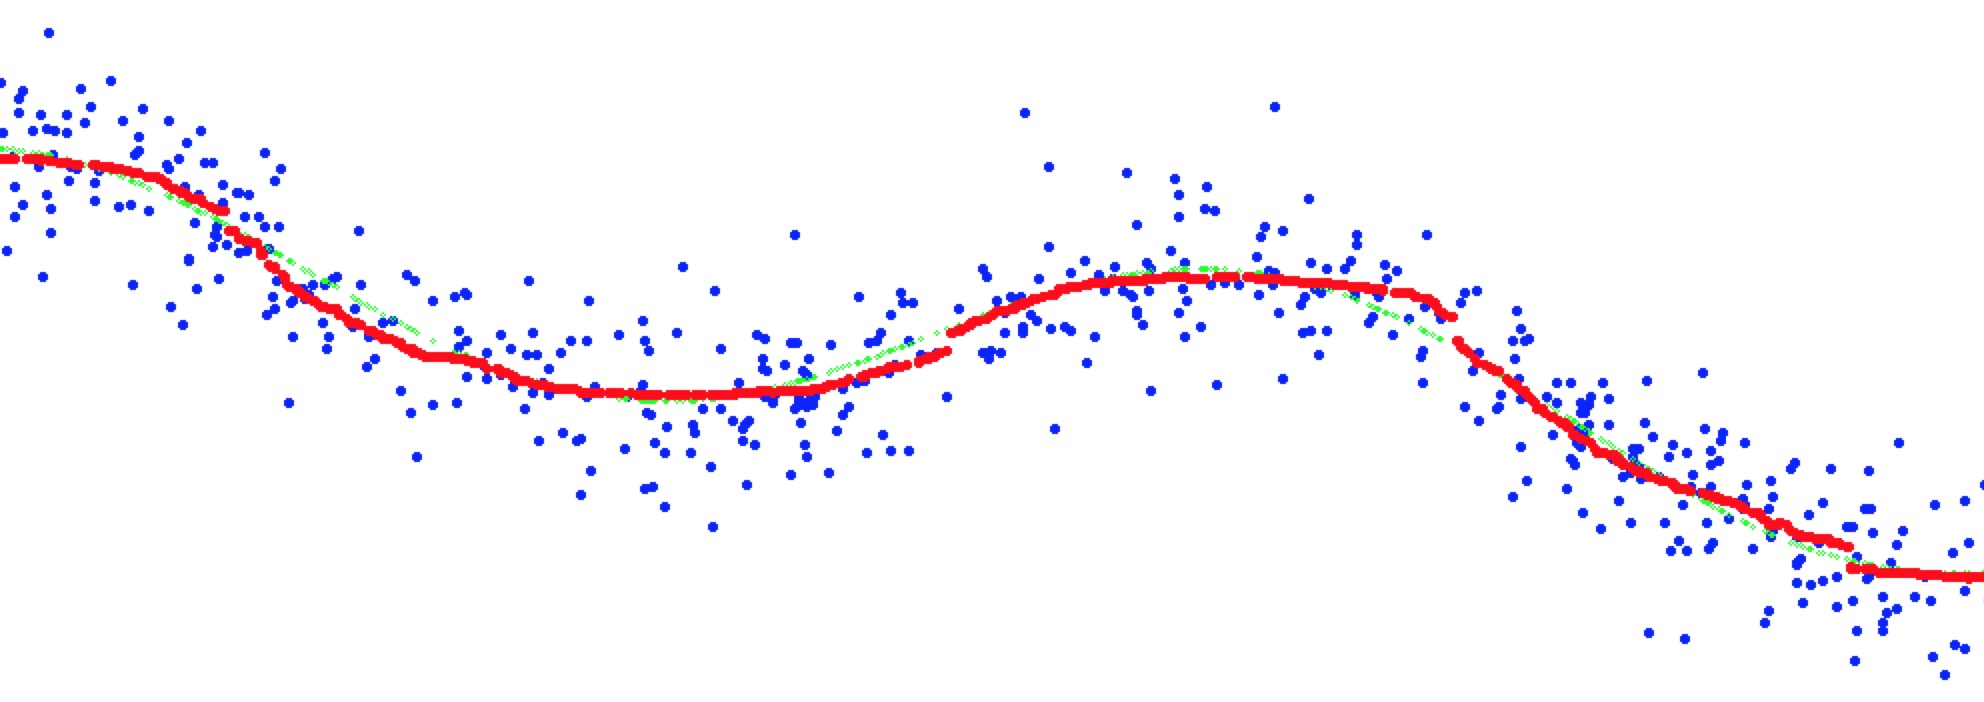
\includegraphics[width=0.6\textwidth]{./mypic/随机蕨回归实验5.jpg} 
	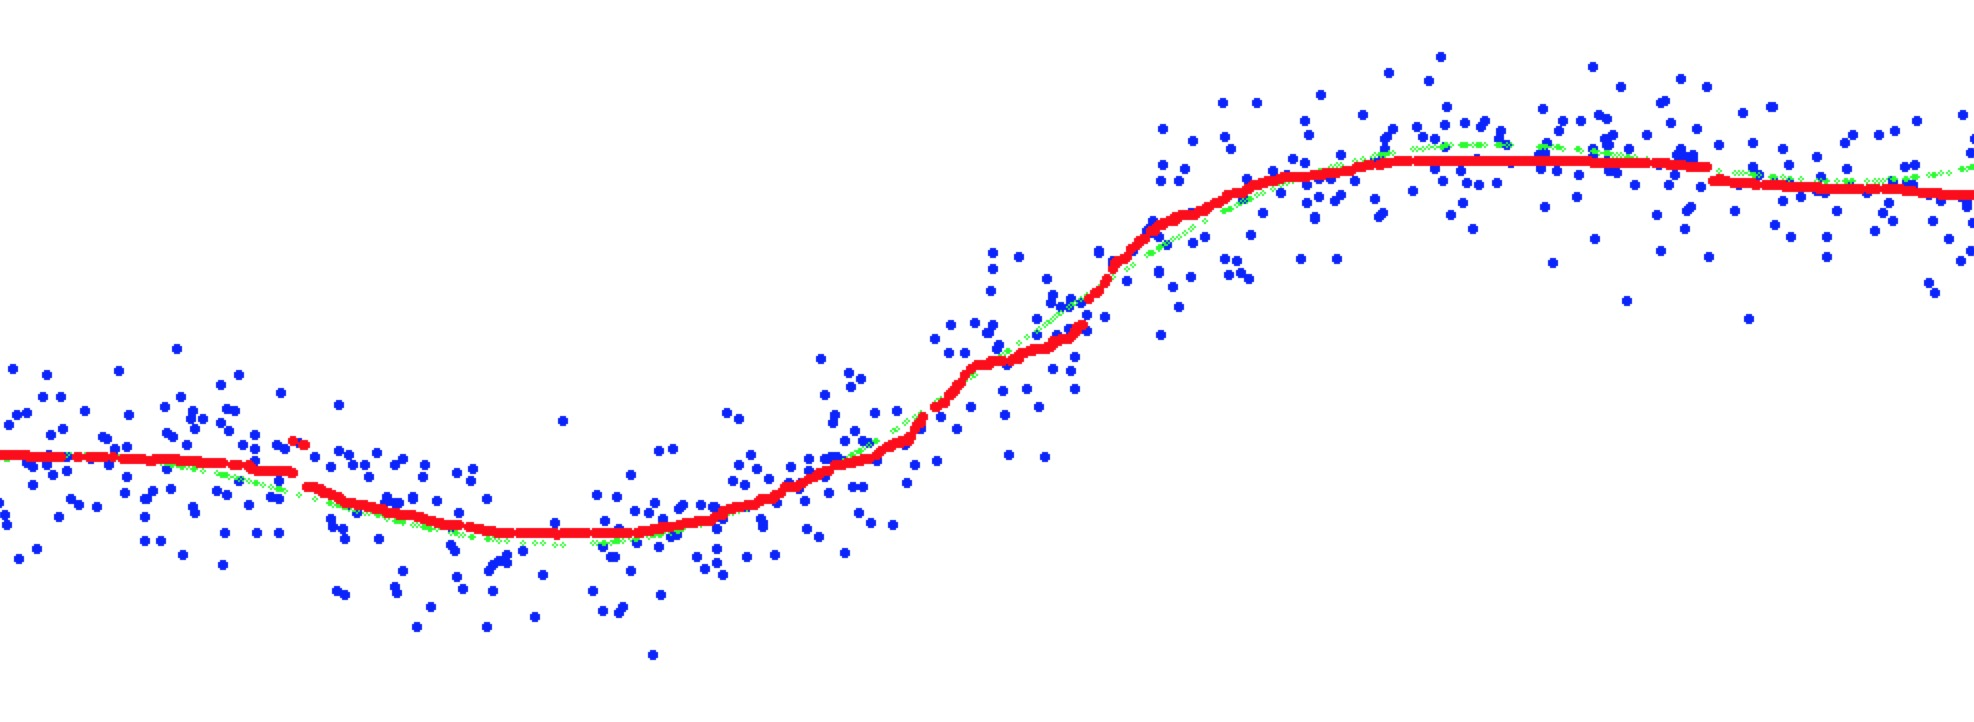
\includegraphics[width=0.6\textwidth]{./mypic/随机蕨回归实验6.jpg} 
	% 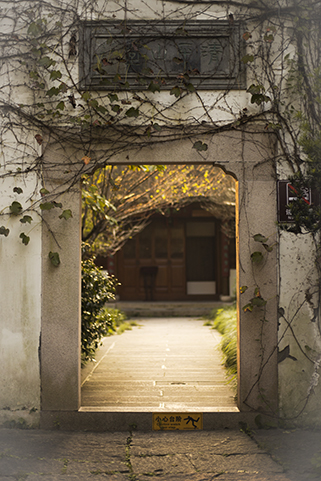
\includegraphics[scale=1.0]{./Pictures/test.jpg} 
	\caption{随机蕨回归实验可视化结果} 
\end{figure}

除此之外,本文还将该随机蕨回归算法应用到人脸特征点定位这个更为复杂的回归问题中去,同样也取得了非常不错的表现。由于该实验涉及一些与本文相关度不高的中间步骤,因此具体实验细节在此不作详述,仅给出实验最后得到的人脸特征点定位结果。图2-5中红色圆点表示通过随机蕨回归器得到的人脸特征点定位结果。该实验中涉及的随机蕨回归模型具有高达1000维度输入以及136维度的回归目标,具有极高的回归复杂度。其优良的表现再次证明了随机蕨回归算法的可行性。

并且,本文将该人脸特征点定位算法结果与现有最为优秀的几个算法进行了比较。通过在300-W数据集\cite{sagonas2013semi}上,采用瞳孔间距正则化误差作为评价标准\cite{belhumeur2013localizing}\cite{cao2014face},本文得到如表2-2所示的结果。从表2-2可以看出,本文算法相比于ESR\cite{cao2014face}、SDM\cite{xiong2013supervised}、LBF fast\cite{ren2014face}这三种算法有更小的误差(其中300-W数据集包含一般数据集和复杂数据集两个部分),并且在算法效率上仅次于LBF fast。此实验中其他三种算法的实验结果均引用于文章[\citenum{ren2014face}],对于精度对比没有影响,但本文算法的帧率测试由于实验平台不同,仅供参考(本文实验环境为2.2GHz Intel Core i7单进程处理器)。该实验可以表明,改进后的随机蕨算法不光具有较好的拟合能力,同时也具备较高的计算效率。

\begin{figure}[htb]
	\centering 
	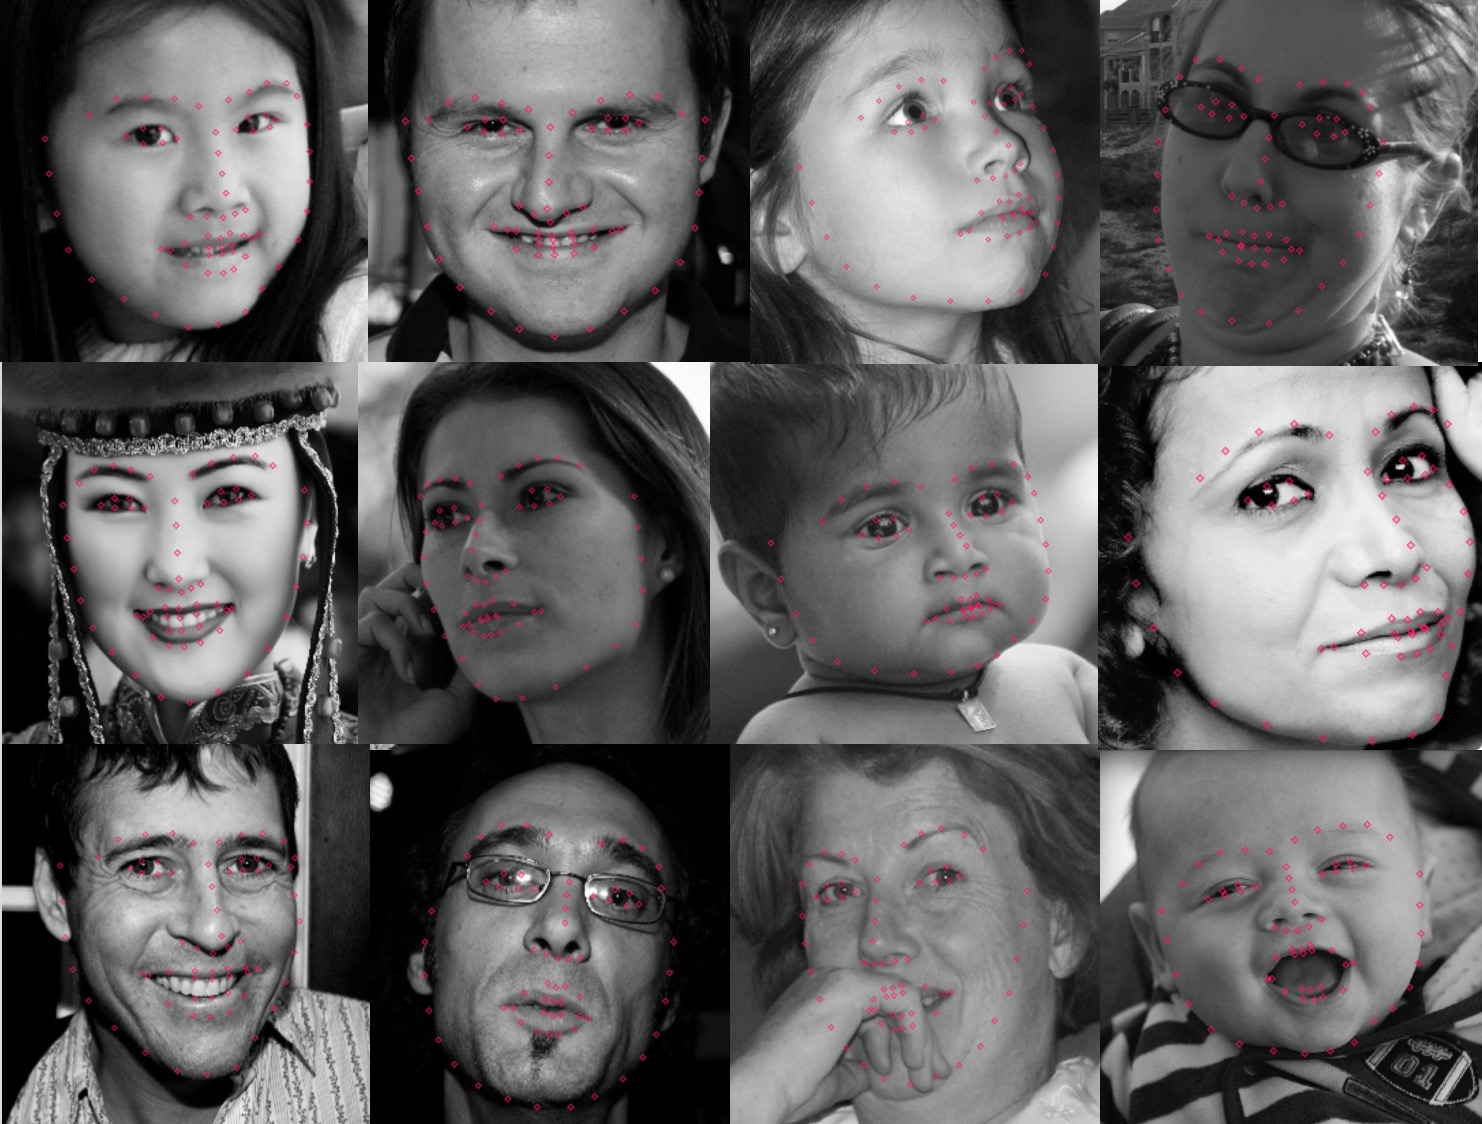
\includegraphics[width=\textwidth]{./mypic/人脸特征点定位实验.jpg} 
	% 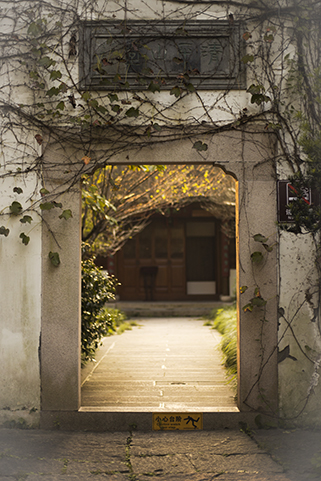
\includegraphics[scale=1.0]{./Pictures/test.jpg} 
	\caption{人脸特征点定位实验结果} 
\end{figure}

\begin{table}[htb]
	\zihao{5}
	\caption{300-W数据集上人脸特征点定位算法对比} 
	% \label{Tabkeyword}
	\centering 
	\begin{tabular}[t]{
		% |c|l|r|p{4cm}|} 
		ccccccc} 
		\toprule
		算法 & 全数据集误差 & 一般数据集误差 & 复杂数据集误差 & 帧率(FPS)\\ 
		\midrule
		ESR\cite{cao2014face} & 7.58 & 5.28 & 17.00 & 120 \\
		SDM\cite{xiong2013supervised} & 7.52 & 5.6 & 15.4 & 70 \\
		LBF fast\cite{ren2014face} & 7.37 & 5.38 & 15.5 & 3100 \\
		Ours & 6.94 & 4.93 & 15.18 & 476 \\
		\bottomrule
	\end{tabular}
\end{table}


\subsection{对大噪声干扰下的随机蕨算法验证} % 

大噪声干扰下的随机蕨算法验证实验由于与本文第四章实验有较多相互依赖的交集,因此对于该问题的实验验证将在4.6节中进行展开,此处不再详细讨论。


\section{本章小节}
本章旨在充分开发随机蕨算法的潜能,通过改造整理,先是总结出经典随机蕨算法应用于回归问题的改进方法,再进一步结合实际问题中存在大噪声干扰下随机蕨算法不够鲁棒的情况,提出掩码机制下的随机蕨回归算法。最后还通过实验验证了随机蕨算法在非线性回归问题下的拟合能力,通过人脸特征点定位这个具有非常大挑战性的回归问题,证实了本章提出的随机蕨回归算法具有较好的实用性以及高效性。























